% =============================================================================
%  UML 2.5 Activity Diagram: Multi-objective Iterative Domain Contraction
%  Linear top-to-bottom main column; loop-back via the left margin.
%  Compile:  pdflatex fig_idc_activity_mo.tex
% =============================================================================
\documentclass[border=4pt,tikz]{standalone}
\usetikzlibrary{positioning,shapes.geometric,shapes.misc,arrows.meta,calc,fit}

\begin{document}
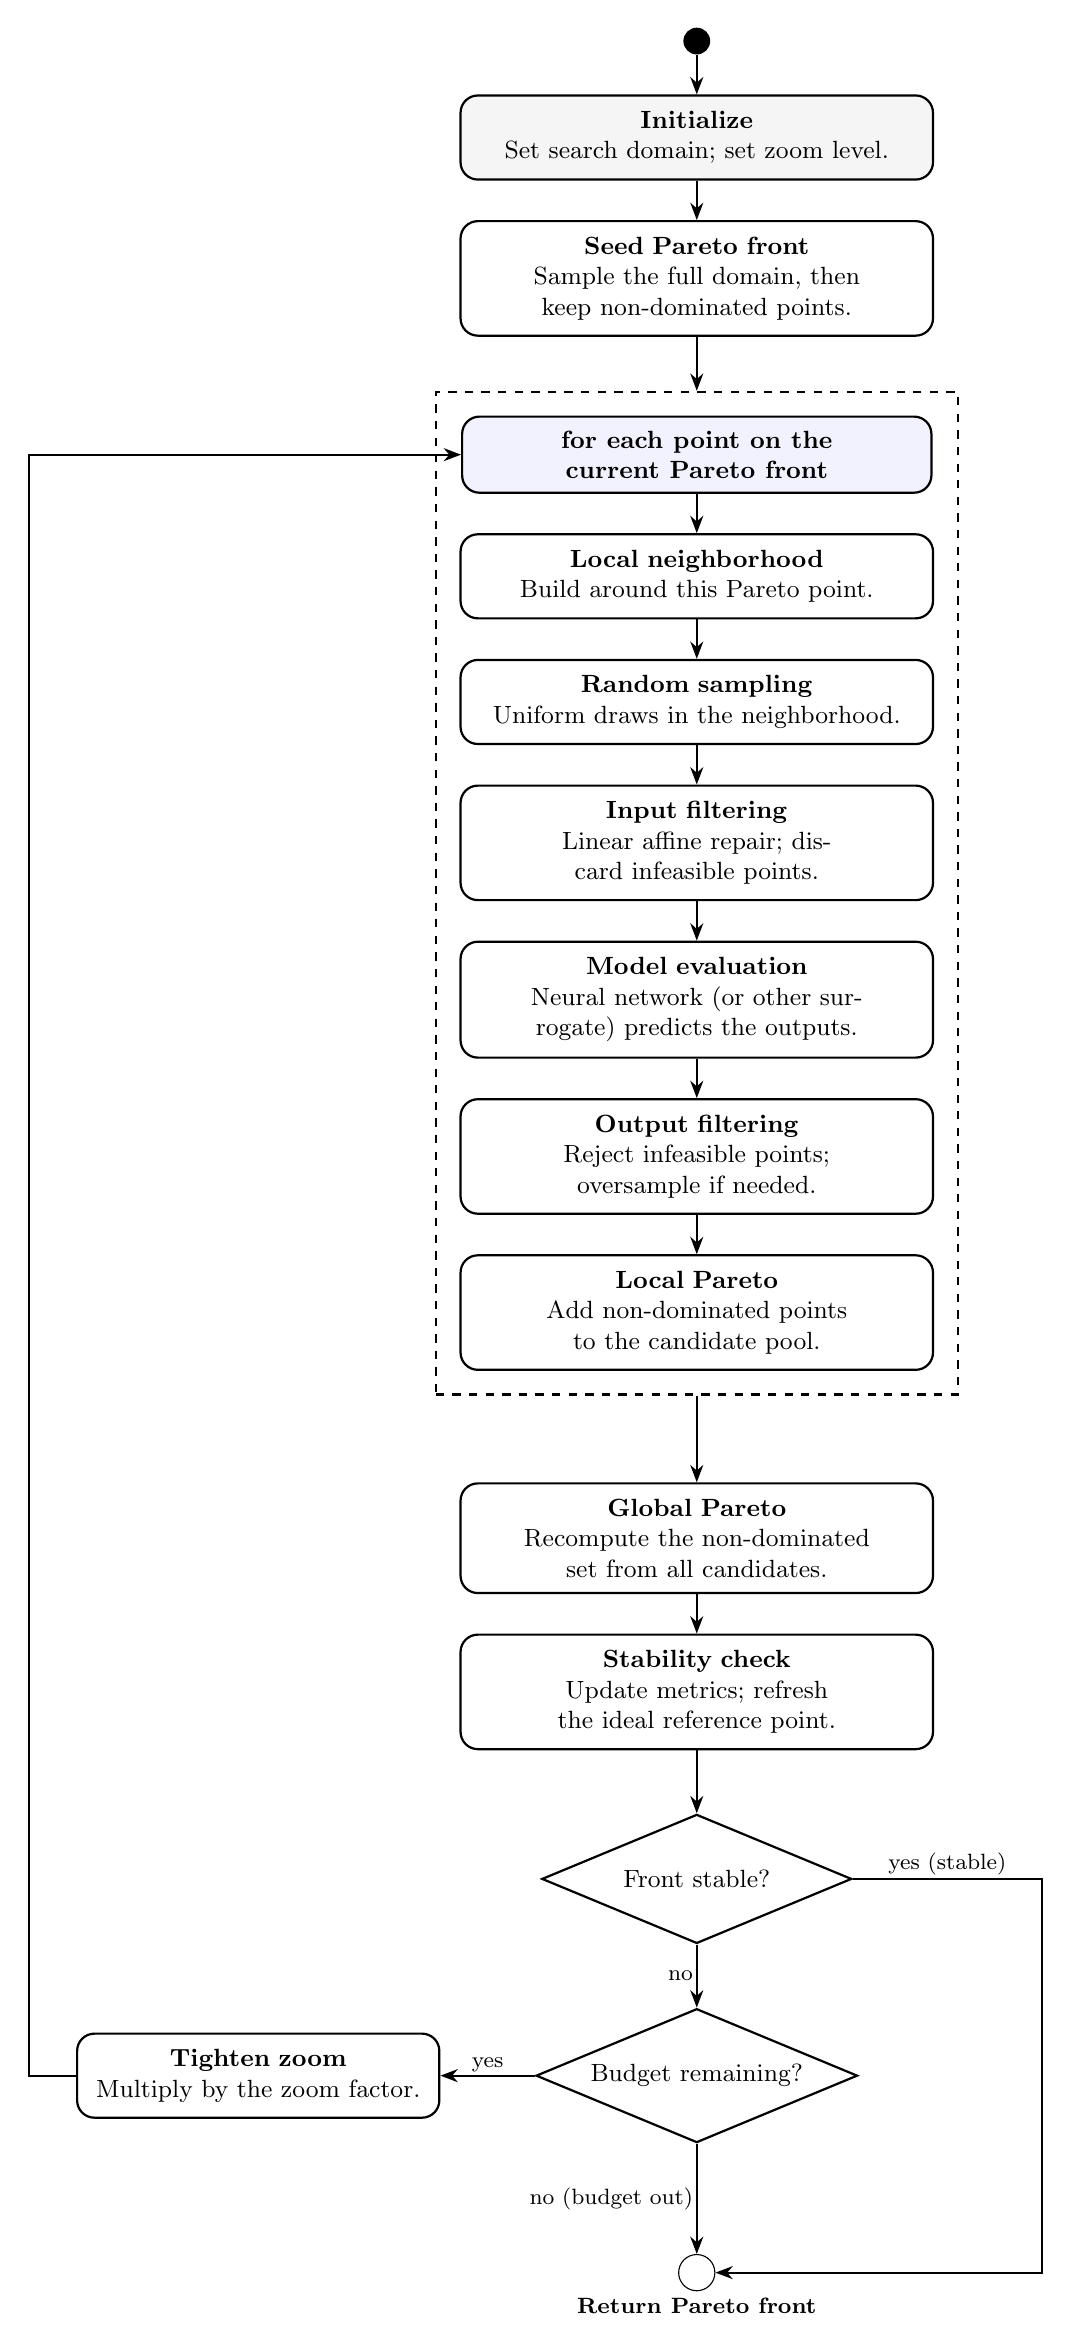
\begin{tikzpicture}[
    font=\small,
    >={Stealth[length=2.2mm]},
    node distance=5mm and 9mm,
    initial/.style   = {circle, fill=black, minimum size=3.4mm, inner sep=0pt},
    final/.style     = {circle, draw, minimum size=4.6mm, inner sep=0pt,
                        label={[anchor=center]center:{\large$\bullet$}}},
    action/.style    = {rectangle, rounded corners=2.2mm, draw, thick,
                        align=center, minimum height=8mm, minimum width=58mm,
                        inner sep=2.0mm, text width=56mm},
    sideaction/.style= {rectangle, rounded corners=2.2mm, draw, thick,
                        align=center, minimum height=8mm, minimum width=44mm,
                        inner sep=2.0mm, text width=42mm},
    init/.style      = {rectangle, rounded corners=2.2mm, draw, thick,
                        align=center, minimum height=8mm, minimum width=58mm,
                        inner sep=2.0mm, fill=black!4, text width=56mm},
    loopheader/.style= {rectangle, rounded corners=2.2mm, draw, thick,
                        align=center, minimum height=7mm, minimum width=58mm,
                        inner sep=1.8mm, fill=blue!5, text width=56mm,
                        font=\small\bfseries},
    decision/.style  = {diamond, draw, thick, align=center, aspect=2.4,
                        inner sep=0.6mm, text width=30mm},
    flow/.style      = {-{Stealth[length=2.2mm]}, thick},
    label/.style     = {font=\footnotesize, inner sep=1pt},
    frag/.style      = {rectangle, draw, dashed, thick, inner sep=3mm,
                        rounded corners=0pt}
]

% --- Main column (top to bottom) --------------------------------------------
\node[initial]                                  (start) {};
\node[init,    below=of start]                  (init)
  {\textbf{Initialize}\\
   Set search domain; set zoom level.};

\node[action,  below=of init]                   (seed)
  {\textbf{Seed Pareto front}\\
   Sample the full domain, then keep non-dominated points.};

% Per-Pareto-point loop region
\node[loopheader, below=10mm of seed]           (forj)
  {for each point on the current Pareto front};

\node[action,  below=of forj]                   (neigh)
  {\textbf{Local neighborhood}\\
   Build around this Pareto point.};

\node[action,  below=of neigh]                  (random)
  {\textbf{Random sampling}\\
   Uniform draws in the neighborhood.};

\node[action,  below=of random]                 (inputf)
  {\textbf{Input filtering}\\
   Linear affine repair; discard infeasible points.};

\node[action,  below=of inputf]                 (eval)
  {\textbf{Model evaluation}\\
   Neural network (or other surrogate) predicts the outputs.};

\node[action,  below=of eval]                   (outf)
  {\textbf{Output filtering}\\
   Reject infeasible points; oversample if needed.};

\node[action,  below=of outf]                   (local)
  {\textbf{Local Pareto}\\
   Add non-dominated points to the candidate pool.};

\node[frag, fit=(forj)(neigh)(random)(inputf)(eval)(outf)(local)] (region) {};

% After the expansion region
\node[action,  below=11mm of region]            (globalpf)
  {\textbf{Global Pareto}\\
   Recompute the non-dominated set from all candidates.};

\node[action,  below=of globalpf]               (stab)
  {\textbf{Stability check}\\
   Update metrics; refresh the ideal reference point.};

\node[decision,below=8mm of stab]               (conv)
  {Front stable?};

\node[decision,below=8mm of conv]               (max)
  {Budget remaining?};

\node[final,   below=14mm of max]               (end) {};
\node[label,   below=0.5mm of end]
  {\textbf{Return Pareto front}};

% --- Side branch (left): Tighten zoom ---------------------------------------
\node[sideaction, left=12mm of max]             (zoom)
  {\textbf{Tighten zoom}\\
   Multiply by the zoom factor.};

% --- Flows -------------------------------------------------------------------
\draw[flow] (start)        -- (init);
\draw[flow] (init)         -- (seed);
\draw[flow] (seed)         -- (region.north);

\draw[flow] (forj)         -- (neigh);
\draw[flow] (neigh)        -- (random);
\draw[flow] (random)       -- (inputf);
\draw[flow] (inputf)       -- (eval);
\draw[flow] (eval)         -- (outf);
\draw[flow] (outf)         -- (local);

\draw[flow] (region.south) -- (globalpf);
\draw[flow] (globalpf)     -- (stab);
\draw[flow] (stab)         -- (conv);

% Decisions: "no" labels on the LEFT
\draw[flow] (conv) -- node[label,left]{no} (max);
\draw[flow] (max)  -- node[label,left]{no (budget out)} (end);

% Termination from stability: bend RIGHT, drop down, enter end from the east
\draw[flow] (conv.east) -- node[label,above]{yes (stable)}
           ++(24mm,0) |- (end.east);

% Loop-back: D2.west -> zoom (left), then up the left margin to region top
\draw[flow] (max.west) -- node[label,above]{yes} (zoom.east);
\draw[flow] (zoom.west) -- ++(-6mm,0) |- (forj.west);

\end{tikzpicture}
\end{document}
